%!TEX encoding = UTF-8 Unicode
\section{Description of the Project}
\label{sec:Architecture}
%- Como pensam abordar a tese tendo em conta o problema, as contribuicoes a que propoe a dar e a arquitectura definida.
%- Descricao de alto nivel da arquitectura do sistema: Arquitectura do SW explicando os principais componentes e as funcoes que executam.
%- Como procederam as escolhas das ferramentas, linguagens de programcao, ambientes de desenvolvimento, hardware
%- Como prevem desenvolver a arquitectura proposta: por onde vao comecar. Como vao integrar os componentes, que dificuldades esperam encontrar e que estrategias planeam para as ultrapassar.
\noindent Based on the reviewed works, the solution proposed in this section is to develop and implement a novel architecture which will provide mobility support to fog nodes as well as to end devices in a simulation toolkit. Besides, it will also optimize the decision-making of migration by implementing multi-objective decisions into the algorithm.\\

\subsection{Simulation toolkit}
\noindent Based on Table \ref{tab:toolkits}, it can clearly be observed that most of the existing simulation toolkits are CloudSim-based. More recent works, in fog computing, have begun to implement their investigation work in iFogSim, which is also based on CloudSim. Moreover, recently some other simulators have been proposed as extensions to iFogSim. Once such attention has been given to this ``family'' of simulators, which implies a a larger community, information and documentation, compared to other isolated simulators, our work will be based on iFogSim.\\
\noindent\tab On the one hand, iFogSim already has really fortunate characteristics. For instance, it has built-in energy (based on CPU utilization), cost (depending on memory, storage, bandwidth and CPU utilization), application (defining deadlines for modules and applications) and communication models (defining delays and bandwidth). Also, it already supports virtualization techniques, namely the use of VMs. Moreover, this simulator supports DDF programming model, where different modules may be deployed in different machines, creating dependencies between them. This is, an application module at a given machine is responsible for processing all data generated from modules hosted at machines bellow in the hierarchy. On the other hand, this simulator has some minor negative points compared with other simulators (refer to Table \ref{tab:toolkits}), however those are not critical. For example, the built-in communication model is unrealistic by disregarding low-level network issues such as link errors, congestion-related losses or management between densely collocated devices. However, these can be treated as high-level attributes like latency or bandwidth of connections. Moreover, as berofe mentioned, GreenCloud is a more fine-grained simulator in what respects to energy consumption. However in iFogSim, energy models are able to vary according to the CPU usage [implementar com envio e receção de dados!!].\\
\noindent\tab Despite the above mentioned, iFogSim still has some drawbacks, namely: it does not provide communication between fog nodes at the same level; rather it only provides parent-child communication. This feature is of most importance as discussed before (e.g., to implement an architecture based on fog colonies). Moreover it does not allow mobility of fog nodes nor end-devices and its application placement is static; does not consider any dynamic environment (although it already provides interfaces to ease this implementation).\\

\subsection{Data Placement Optimization}
\noindent Based on iFogSim, in order to achieve the desired objectives, firstly is necessary to implement ``horizontal'' communication between fog nodes.\\
\noindent\tab At the beginning of each simulation, iFogSim executes a placement strategy which is responsible to distribute the miscellaneous of modules composing an application among the available fog nodes. These nodes are deployed in a hierarchical manner where each fog node has a parent (except for the cloud). Thus, a path is composed by the intermediate fog nodes and links between them and the cloud and the gateway (fog node which is connected to the sensors and/or actuators). This strategy, favors the placement of modules closer to the end-devices (where the raw data is generated). As already mentioned modules have some dependencies (i.e. the data from one module may be the input of other model). Specifically, this strategy goes for each fog node in a given path search for what are the modules that can be placed (i.e. all their predecessors/dependencies were already placed in south fog nodes). Then, for each one of these modules, it will verify if the current node is able to host it, based on the available CPU [na memoria não? qt memoria cada modulo??]. If not, the module is transferred vertically in the hierarchy until some machine is able to host it. This is poorly efficient in terms of load balancing, QoS guarantees nor search complexity. It is worth noting that this strategy is preformed before the actual simulation begin, thus it does not take into account the real migration problems. Is a very basic static placement.\\
\noindent\tab The above strategy uses the attribute 'parent id' preform this search. Our aim is to search not only vertically but also along all neighborhoods. In a first stage, as iFogSim does not considers geographical positioning of fog servers, we will assume that fog nodes at the same level, are in the close vicinity. Once this is achieved, our objective is to somehow divide the whole system. As already mentioned this algorithm is not very efficient. It may work for systems composed by few fog nodes, but as the system grows to a bigger scale, it would not be feasible. Thus, in order to provide scalability, we aim to divide the search problem into small systems (e.g., as fog colonies does). To do so, we aim so implement graph partitioning functionality that iFogSimWithDataPlacement simulator has already implemented. Specifically this feature is implemented using three components. First, the graph modeling engine which creates an undirected graph where vertices represent fog nodes and edges model physical links. Then, the graph weighting engine that is responsible allocate weights for both vertices (based on the number of data items produced produced in each fog node) and edges (based on the number of data flows passing through these links). Finally, the graph partition engine is responsible to apply a k-way partitioning method to divide it into k sub-graphs using Metis \cite{METISSer49:online} using the typical criterias: balancing the vertex weights between sub-graphs, and minimizing the sum of cut edges weights. We also intend to compare this approaches using different criterias to perform partitioning such as the end to end latency, phisical distance or network distance (i.e. number of hops).\\
\noindent\tab After this first stage, we are now able to implement and test some algorithms proposed in the reviewed literature (refer to Section \ref{sec:Migration}). This would take into account the available parameters in iFogSim to minimize latencies and some other objectives such as energy, cost, bandwidth and, afterwards, jointly consider them all. To allow this optimization iFogSim already has built-in some valuable characteristics in fog nodes, as presented bellow:
\begin{center}
	\begin{varwidth}[t]{.5\textwidth}
	\begin{itemize}
		\item costPerSecond (Price/CPU unit)
		\item costPerMem
		\item costPerStorage
		\item costPerBw
		\item uplinkLatency
	\end{itemize}
\end{varwidth}% <---- Don't forget this %
\hspace{4em}% <---- Don't forget this %
\begin{varwidth}[t]{.5\textwidth}
	\begin{itemize}
		\item uplinkBandwidth
		\item downlinkBandwidth
		\item idlePower
		\item busyPower
	\end{itemize}
\end{varwidth}
\end{center}
As such, it will be possible to model the minimization problems and solve them with the algorithms presented in Section \ref{sec:Algoritms}. The objective is to evaluate their performance in terms of both actual optimization and computational complexity. Note that in this stage we are facing a static environment where the optimization is performed before the actual simulation.

\subsection{Mobility support}
After the above implementation, the aim is to provide mobility support. For this propose MyiFogSim, which is also an extension of iFogSim, already provide some important features. It provides mobility support to end devices through migration of virtual machines between fog nodes. On the one hand, their approach introduces the migration policy which is responsible to answer to \textit{when} the VM should be migrated using users movement (i.e. position, speed, and direction). On the other hand, upon the decision to migrate, they have introduced the migration strategy which defines \textit{where} and \textit{how} the VM should it be migrated. While the latter regards to the type of migration (i.e. non-live container/VM migration or VM live migration using post copy), the former uses some simple strategies to define the fog node destination such as shortest distance or lowest latency. However, as some review works have shown (e.g., \cite{sun2016primal,zhang2016segue}), these greedy strategies are not perfect at all, and other parameters have to be taken into account. Hence, this work intends to implement some work already preformed but not all. Besides, this work also aims to provide fog servers mobility.\\
After this implementation, is also objective to adjust the previous optimization to take into account, now, both users and fog nodes mobility and lastly to take into account mobility patterns.

\subsection{Architecture}
Based on the above mentioned our implementation consists in apply the architecture presented in figure \ref{sw_architecture}. Grey classes are from iFogSim and CloudSim simulators, yellow classes are from MyiFogSim simulator and the green ones are from iFogSimWithDataPlacement. Note that those classes are the presented in the corresponding papers, being the most important ones in their implementations. Our implementation will be focused in the white classes. It is worth mentioning that both MyiFogSim and iFogSimWithDataPlacement, as shown in Table \ref{tab:toolkits}, do not have documentation and some error were already found. Therefore, it is high unpredictable to estimate the efforts that it will require to aggregate their implementations.

\begin{figure} [t]
	\centering
	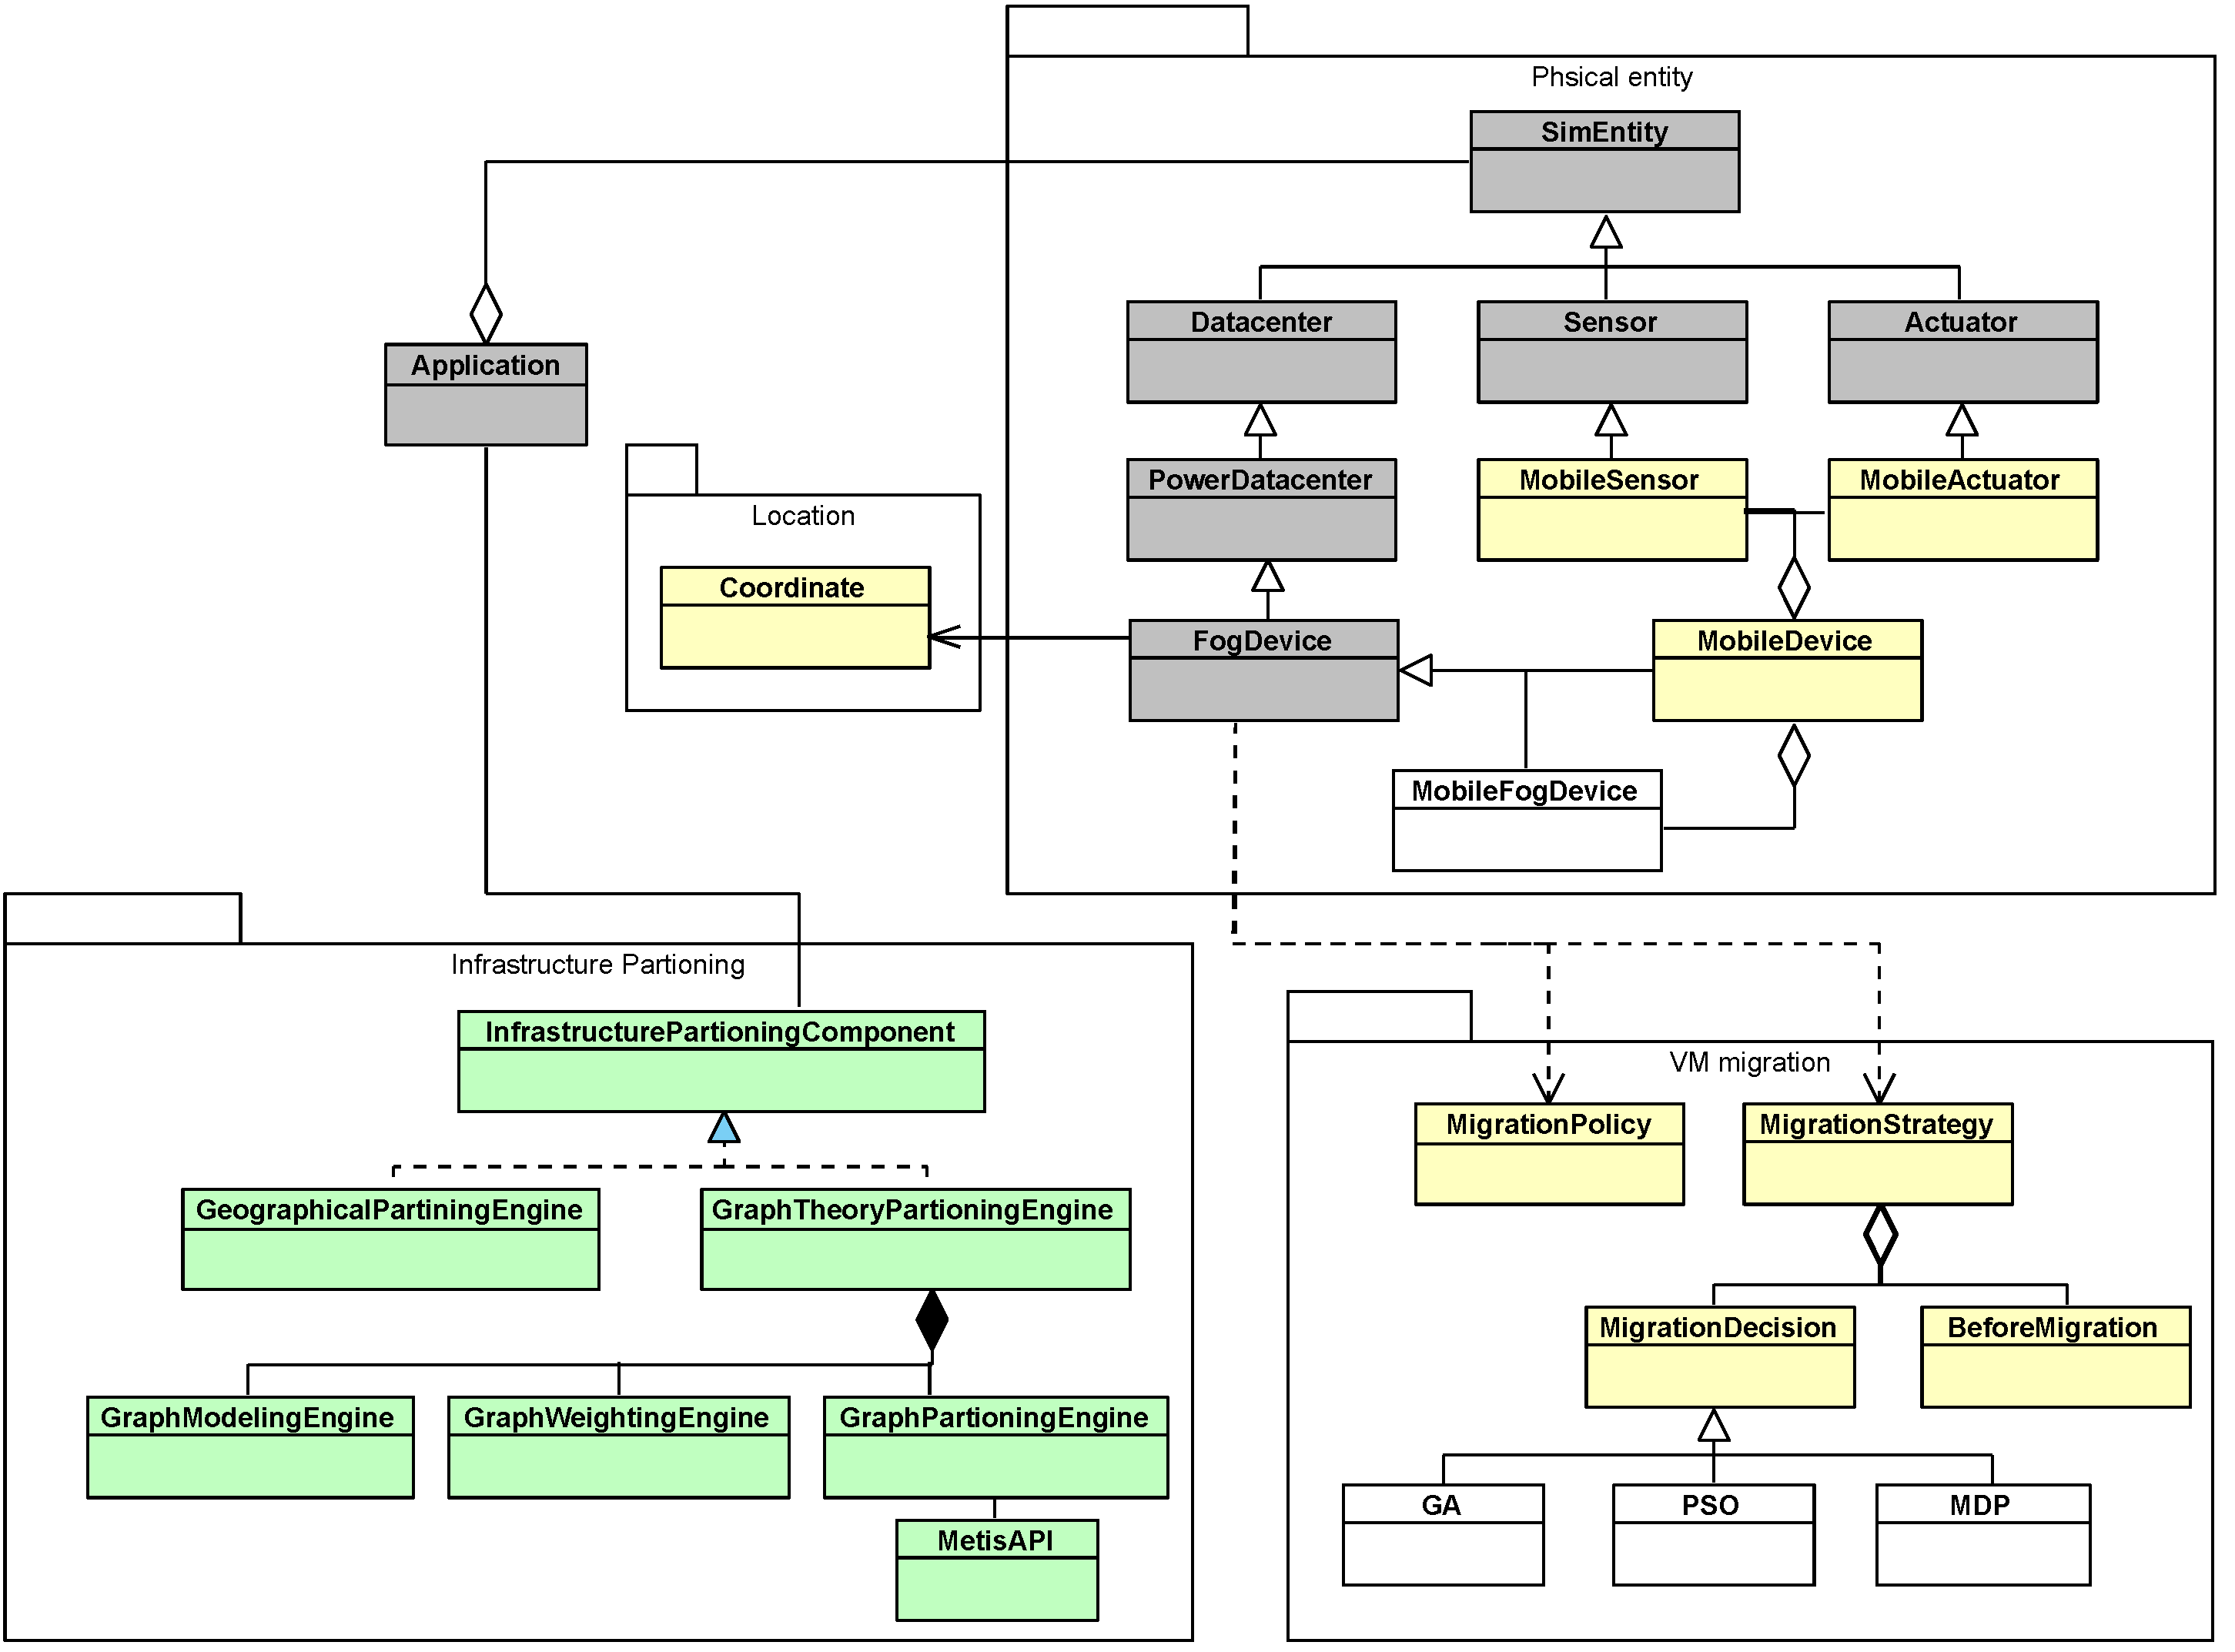
\includegraphics[width=\textwidth]{images/sw_architecture/sw_architecture}
	\caption{UML Class diagram of the main added functionalities.}
	\label{sw_architecture}
\end{figure}

As it can be seen, our work will implement four main classes, namely: MobileFogDevice, GA, PSO and MDP. The MobileFogDevice class will extend from FogDevice. Therefore, it will inherit all its attributes and methods. Besides, it will have a few similarities to the MobileDevice from MyiFogSim such as the direction, speed and geographical position. The three latter will focus on implementing the algoritms of optimization explained in Section \ref{sec:Migration}. Relatively to the recalculation of the optmization problem, it cannot be defined how it will be done now. This is because, we first need to evaluate their behavior in terms of computational complexity and execution time. Only after this process we will be able to define it. However there are some options to do so. Based on the review literature we have three options. The first, proposed by MyiFogSim, is to recalculate only when the user is predicted to go out of range from a base station. Based on its position, direction and speed we can predict an handover. When this is verified, the algorithm is executed to compute the best placement to its VM (compute the cloudlet destination). Their approach is a single user-centric approach, therefore it does not take into account system efficiency what is a bad approach as already explained. Other options were already proposed in the literature. For instance, the algorithm may be recalculated periodically, but the optimal time interval is never proposed (it is only said that it depends on system dynamics). Finally, the third approach, it to only recalculate when a QoS violation is predicted. In the latter, it would evolve several parameters such as server and network states as well as mobility and request patterns. As already stated, there are quite unpredictable time implementations during the implementation of the proposed architecture. Therefore, we do not know if it will be possible to implement mobility and request patterns and we may be restricted to the first two approaches.\\

\subsection{Optimization Algoritms}
As already mentioned, we intend to implement and test some of the proposed algorithms in the reviewed literature. From the panoply of solvers, we intend to study the behavior of the three presented bellow and, later, depending on the time available, more algorithms may be tested.

\subsubsection{Genetic Algorithm}
GA is an adaptive heuristic search algorithm. It is based on the idea of natural selection and genetics. Specifically, it is an iterative random search which is able to provide high-quality solutions for optimization problems and search problems.\\
\noindent\tab The algorithm has an arbitrary number of individuals composing the population. During the process, each iteration is characterized by a generation of individuals (whith the same size of population), representing a point in search space and possible solution. Yet, for each iteration, it is simulated the process of natural selection or ``survival of the fittest''. Each individual has a chromosome with genes. By evaluate them, it is possible to define its fitness score. Using this score, there are three operations in the creation of the next generation, namely: the selection operator which selects the individuals that will be part of the next generation, the crossover operator which represents mating between two individuals, resulting in a new individual with a chromosome composed by random genes from the two parents, and, finally, the mutation operator that will randomly introduce genes in the individuals resulting from the crossover operator to maintain the diversity in population to avoid the premature convergence \cite{whitley1994genetic}.

\subsubsection{Particle Swarm Optimization}

\subsubsection{Markov Decision Process}

%A arquitetura dos Buses é boa (APs com várias cloudlets etc....)

%Starting from available simulators a significant programming effort is required to obtain a simulation tool meeting the actual needs.
%Simply applying existing radio access-oriented MM (mobility management) schemes leads to poor performance mainly due to the co-provisioning of radio access and computing services of the MEC-enabled (mobile edge computing) BSs (base stations).
%On a self-driving vehicle, are estimated to generate about 1GB data per second \cite{angelica2013google}. As the number of features grow, the data deluge grows out of control. Moreover, these types of systems, where people's lives depends on it, are hard real-time what means that it is absolutely imperative that all deadlines are met. Offloading tasks to fog nodes will be the best solution, once a big effort in mobility support has been done through the migration of VMs using cloudlets \cite{lopes2017myifogsim}. Also, in this context, Puliafito et al. address three types of applications where fog is required, namely, citizen's healthcare, drones for smart urban surveillance and tourists as time travellers \cite{puliafito2017fog}, addressing the needs of low latency and mobility support.\\